% Тип документа
\documentclass[a4paper,12pt]{extarticle}

% Шрифты, кодировки, символьные таблицы, переносы
\usepackage{cmap}
\usepackage[T2A]{fontenc}
\usepackage[utf8x]{inputenc}
\usepackage[russian]{babel}

% Это пакет -- хитрый пакет, он нужен но не нужен
\usepackage[mode=buildnew]{standalone}

\usepackage
	{
		% Дополнения Американского математического общества (AMS)
		amssymb,
		amsfonts,
		amsmath,
		amsthm,
		% misccorr,
		% 
		% Графики и рисунки
		wrapfig,
		graphicx,
		subcaption,
		float,
		tikz,
		% tikz-3dplot,
		caption,
		csvsimple,
		color,
		booktabs,
		pgfplots,
		pgfplotstable,
		geometry,
		% 
		% Таблицы, списки
		makecell,
		multirow,
		indentfirst,
		%
		% Интегралы и прочие обозначения
		ulem,
		esint,
		esdiff,
		% 
		% Колонтитулы
		fancyhdr,
	}  


% Обводка текста в TikZ
\usepackage[outline]{contour}

% Увеличенный межстрочный интервал, французские пробелы
\linespread{1.3} 
\frenchspacing 

 
\usetikzlibrary
	{
		decorations.pathreplacing,
		decorations.pathmorphing,
		patterns,
		calc,
		scopes,
		arrows,
		fadings,
		through,
		shapes.misc,
		arrows.meta,
		3d,
		quotes,
		angles,
		babel
	}


\tikzset{
	force/.style=	{
		>=latex,
		draw=blue,
		fill=blue,
				 	}, 
	%				 	
	axis/.style=	{
		densely dashed,
		blue,
		line width=1pt,
		font=\small,
					},
	%
	th/.style=	{
		line width=1pt},
	%
	acceleration/.style={
		>=open triangle 60,
		draw=magenta,
		fill=magenta,
					},
	%
	inforce/.style=	{
		force,
		double equal sign distance=2pt,
					},
	%
	interface/.style={
		pattern = north east lines, 
		draw    = none, 
		pattern color=gray!60,
					},
	cross/.style=	{
		cross out, 
		draw=black, 
		minimum size=2*(#1-\pgflinewidth), 
		inner sep=0pt, outer sep=0pt,
					},
	%
	cargo/.style=	{
		rectangle, 
		fill=black!70, 
		inner sep=2.5mm,
					},
	%
	caption/.style= {
		midway,
		fill=white!20, 
		opacity=0.9
					},
	%
	}

\newenvironment{tikzpict}
    {
	    \begin{figure}[htbp]
		\centering
		\begin{tikzpicture}
    }
    { 
		\end{tikzpicture}
		% \caption{caption}
		% \label{fig:label}
		\end{figure}
    }


\newcommand{\vbLabel}[3]{\draw ($(#1,#2)+(0,5pt)$) -- ($(#1,#2)-(0,5pt)$) node[below]{#3}}
\newcommand{\vaLabel}[3]{\draw ($(#1,#2)+(0,5pt)$) node[above]{#3} -- ($(#1,#2)-(0,5pt)$) }

\newcommand{\hrLabel}[3]{\draw ($(#1,#2)+(5pt,0)$) -- ($(#1,#2)-(5pt,0)$) node[right, xshift=1em]{#3}}
\newcommand{\hlLabel}[3]{\draw ($(#1,#2)+(5pt,0)$) node[left, xshift=-1em]{#3} -- ($(#1,#2)-(5pt,0)$) }



\newcommand\zi{^{\,*}_i}
\newcommand\sumn{\sum_{i=1}^{N}}

\tikzset{
	coordsys/.style={scale=1.8,x={(1.1cm,-0cm)},y={(0.5cm,1cm)}, z={(0cm,0.8cm)}},
	coordsys/.style={scale=1.5,x={(0cm,0cm)},y={(1cm,0cm)}, z={(0cm,1cm)}}, 
	coordsys/.style={scale=1.5,x={(1cm,0cm)},y={(0cm,1cm)}, z={(0cm,0cm)}}, 
}

\usepgfplotslibrary{units}


% Draw line annotation
% Input:
%   #1 Line offset (optional)
%   #2 Line angle
%   #3 Line length
%   #5 Line label
% Example:
%   \lineann[1]{30}{2}{$L_1$}

\newcommand{\lineann}[4][0.5]{%
    \begin{scope}[rotate=#2, blue,inner sep=2pt, ]
        \draw[dashed, blue!40] (0,0) -- +(0,#1)
            node [coordinate, near end] (a) {};
        \draw[dashed, blue!40] (#3,0) -- +(0,#1)
            node [coordinate, near end] (b) {};
        \draw[|<->|] (a) -- node[fill=white, scale=0.8] {#4} (b);
    \end{scope}
}

\newcommand{\lineannn}[4][0.5]{%
    \begin{scope}[rotate=#2, blue,inner sep=2pt, ]
        \draw[dashed, blue!40] (0,0) -- +(0,#1)
            node [coordinate, near end] (a) {};
        \draw[dashed, blue!40] (#3,0) -- +(0,#1)
            node [coordinate, near end] (b) {};
        % \draw[color=white, color=blue] (a) -- node[fill=white, scale=0.8] {#4} (b);
        \draw[->|] (a)++(-0.3,0) -- (a);
        \draw[->|] (b)++(0.3,0) coordinate (xx) -- (b);
        \draw (xx) node[fill=white, scale=0.8, right] {#4};
    \end{scope}
}

% Круговая стрелка относительно центра (дуга из центра)
\tikzset{
  pics/carc/.style args={#1:#2:#3}{
    code={
      \draw[pic actions] (#1:#3) arc(#1:#2:#3);
    }
  },
  dash/.style={
  	dash pattern=on 5mm off 5mm
  }
}

% Среднее <#1>
\newcommand{\mean}[1]{\langle#1\rangle}

\pgfplotsset{
    % most recent feature set of pgfplots
    compat=newest,
}

% const прямым шрифтом
\newcommand\ct[1]{\text{\rmfamily\upshape #1}}
\newcommand*{\const}{\ct{const}}


\usepackage[europeanresistors,americaninductors]{circuitikz}

% Style to select only points from #1 to #2 (inclusive)
\pgfplotsset{select/.style 2 args={
    x filter/.code={
        \ifnum\coordindex<#1\def\pgfmathresult{}\fi
        \ifnum\coordindex>#2\def\pgfmathresult{}\fi
    }
}}


\usepackage{array}



%%%%%%%%%%%%%%%%%%%%%%%%%%%%%%%%%%%%%%%%%%%%%%%%%
\makeatletter
\newif\if@gather@prefix 
\preto\place@tag@gather{% 
  \if@gather@prefix\iftagsleft@ 
    \kern-\gdisplaywidth@ 
    \rlap{\gather@prefix}% 
    \kern\gdisplaywidth@ 
  \fi\fi 
} 
\appto\place@tag@gather{% 
  \if@gather@prefix\iftagsleft@\else 
    \kern-\displaywidth 
    \rlap{\gather@prefix}% 
    \kern\displaywidth 
  \fi\fi 
  \global\@gather@prefixfalse 
} 
\preto\place@tag{% 
  \if@gather@prefix\iftagsleft@ 
    \kern-\gdisplaywidth@ 
    \rlap{\gather@prefix}% 
    \kern\displaywidth@ 
  \fi\fi 
} 
\appto\place@tag{% 
  \if@gather@prefix\iftagsleft@\else 
    \kern-\displaywidth 
    \rlap{\gather@prefix}% 
    \kern\displaywidth 
  \fi\fi 
  \global\@gather@prefixfalse 
} 
\newcommand*{\beforetext}[1]{% 
  \ifmeasuring@\else
  \gdef\gather@prefix{#1}% 
  \global\@gather@prefixtrue 
  \fi
} 
\makeatother
%%%%%%%%%%%%%%%%%%%%%%%%%%%%%%%%%%%%%%%%%%%%%%%%%

\geometry		
	{
		left			=	2cm,
		right 			=	2cm,
		top 			=	3cm,
		bottom 			=	3cm,
		bindingoffset	=	0cm
	}

%%%%%%%%%%%%%%%%%%%%%%%%%%%%%%%%%%%%%%%%%%%%%%%%%%%%%%%%%%%%%%%%%%%%%%%%%%%%%%%



	%применим колонтитул к стилю страницы
\pagestyle{fancy} 
	%очистим "шапку" страницы
\fancyhead{} 
	%слева сверху на четных и справа на нечетных
\fancyhead[R]{\labauthors} 
	%справа сверху на четных и слева на нечетных
\fancyhead[L]{Отчёт по лабораторной работе №\labnumber} 
	%очистим "подвал" страницы
\fancyfoot{} 
	% номер страницы в нижнем колинтуле в центре
\fancyfoot[C]{\thepage} 

%%%%%%%%%%%%%%%%%%%%%%%%%%%%%%%%%%%%%%%%%%%%%%%%%%%%%%%%%%%%%%%%%%%%%%%%%%%%%%%

\renewcommand{\contentsname}{Оглавление}

\usepackage{tocloft}
% \renewcommand{\cftpartleader}{\cftdotfill{\cftdotsep}} % for parts
% \renewcommand{\cftsectiondotsep}{\cftdotsep}% Chapters should use dots in ToC
\renewcommand{\cftsecleader}{\cftdotfill{\cftdotsep}}
%\renewcommand{\cftsecleader}{\cftdotfill{\cftdotsep}} % for sections, if you really want! (It is default in report and book class (So you may not need it).
% ---------
% \newcommand{\cftchapaftersnum}{.}%
% \usepackage{titlesec}
% \titlelabel{\thetitle.\quad}
\usepackage{secdot}
\sectiondot{subsection}
\usepackage{setspace}

\begin{document}

\def\labauthors{Понур К.А., Сарафанов Ф.Г., Сидоров Д.А.}
\def\labgroup{420}
\def\labnumber{3000}
\def\labtheme{Гармонический анализ и синтез периодических сигналов}
\renewcommand{\vec}{\mathbf}
\renewcommand{\Re}{\operatorname{Re}}
\renewcommand{\Im}{\operatorname{Im}}
\renewcommand{\phi}{\varphi}
\renewcommand{\kappa}{\varkappa}
\renewcommand{\hat}{\widehat}
%%%%%%%%%%%%%%%%%%%%%%%%%%%%%%%%%%%%%%%%%%%%%%%%%%%%%%%%%%%%%%%%%%%%%%%%%%%%%%%
\begin{titlepage}

\begin{center}

{\small\textsc{Нижегородский государственный университет имени Н.\,И. Лобачевского}}
\vskip 1pt \hrule \vskip 3pt
{\small\textsc{Радиофизический факультет}}

\vfill

{\Large Отчет по лабораторной работе №\labnumber\vskip 12pt\bfseries \labtheme}
	
\end{center}

\vfill
	
\begin{flushright}
	{Выполнили студенты \labgroup\ группы\\ \labauthors}%\vskip 12pt Принял:\\ Менсов С.\,Н.}
\end{flushright}
	
\vfill
	
\begin{center}
	Нижний Новгород, \the\year
\end{center}

\end{titlepage}


%%%%%%%%%%%%%%%%%%%%%%%%%%%%%%%%%%%%%%%%%%%%%%%%%%%%%%%%%%%%%%%%%%%%%%%%%%%%%%%
\begin{spacing}{1}
\tableofcontents
\end{spacing}
% \setstretch{1.2}
\newpage
%%%%%%%%%%%%%%%%%%%%%%%%%%%%%%%%%%%%%%%%%%%%%%%%%%%%%%%%%%%%%%%%%%%%%%%%%%%%%%%
\section{Введение}
 	Изменяющийся во времени сигнал $S(t)$ называется периодическим, если для него выполняется условие
 	\begin{equation}
 		S(t)=S(t+kT),
 	\end{equation}
 	где $T$-- период изменения, а $k$-- любое целое число
Если периодическая функция $S(t)$ удовлетворяет условиям Дирихле, то есть является огранченной и имеет в пределах одного периода конечное число экстремумов и разрывов, то согласно теореме Фурье онра может быть представлена  виде тригонометричекого ряда, называемого рядом Фурье
\begin{equation}
	\label{eq:1}
	S(t)=\frac{a_0}{2}+\sum_{n=1}^\infty(a_n\cos(n\Omega )+b_n\sin{n\Omega t})
\end{equation}
коэффициенты которго определяются из выражений
\begin{equation}
	\label{eq:2.1}
	a_n=\frac{2}{T}\int\limits_{-\frac{T}{2}}^{\frac{T}{2}}S(t)\cos(n\Omega t )dt
\end{equation}
\begin{equation}
	\label{eq:2.2}
	b_n=\frac{2}{T}\int\limits_{-\frac{T}{2}}^{\frac{T}{2}}S(t)\sin(n\Omega t )dt,
\end{equation}
а угловая частота $\Omega$ связана с периодом $T$ соотношением:
\begin{equation}
	\Omega=\frac{2\pi}{T}
\end{equation}
Пользуясь формулами тригонометрии ряд (\ref{eq:1}) можно записать в виде
\begin{equation}
\label{eq:3}
 	S(t)=\frac{a_0}{2}+\sum_{n=1}^{\infty}A_n\cos(n\Omega t-\theta_n)
 \end{equation} 
 более наглядно определяющем совокупность гармонических составляющих, на которые раскладывается исходная функция $S(t)$. Такая совокупность называется спектром. Для периодических функций спектр является дискретным и состоит из постоянной составляющей, которую можно рассматривать как гарминику с нулевой частотой и амплитудой $A_0=a_0/2$ и бесконечного множества гармонических составляющих с частотами $\omega_n=n\Omega$, кратными основной частоте $\Omega$, амплитудами $A_n$ и начальными фазами $\theta_n$.

 Для наглядности спектры удобно изображать в виде спектральных диаграмм -- амплитудных и фазовых.
 Используя формулу
 \begin{equation}
 	\cos\alpha=\frac{e^{i\alpha}+e^{-i\alpha}}{2}
 \end{equation}
 можно от (\ref{eq:3}) перейти к комплексной форму ряда Фурье
 \begin{equation}
 	\label{eq:4}
 	S(t)=\frac{a_0}{2}+\Re\sum_{n=1}^{\infty}A_ne^{in\Omega t}=\frac{1}{2}\sum_{n=1}^{\infty}A_ne^{in\Omega t}, %как пишется крышечка??
 \end{equation}
 где комплексная амплитуда $A_n=A_ne^{\pi\theta_n}$ содержит информацию об комплексной амплитуде и фазе n-ой гармоники. Сравнивая ряды (\ref{eq:4}) и (\ref{eq:1}) и используя соотношения (\ref{eq:2.1}) и (\ref{eq:2.2}), можно получить формулу для вычисления комплесных амплитуд
 \begin{equation}
 	A_n=\frac{2}{T}\int\limits_{-\frac{2}{T}}^{\frac{T}{2}}
 \end{equation}

 Отметим некоторые свойства рядов Фурье.

 1. Если $S(t)$- четная функция, то в выражении (\ref{eq:1}) $b_n$=0, а в разложении остаются только косинусоидальные члены.

 2. Для нечетной функции $S(t)$ в разложении (\ref{eq:1}), наоборот, лишь коэффициенты $b_n$ отличны от нуля, а в $a_n=0$;

 3. При увеличении периода сигнала $T$ расстояние по оси частот между соседними спектральными компонентами уменьшается, то есть спектр становится более <<плотным>>;
 4. Для импульсных сигналов, у которых промежуток времени, когда сигнал отличен от нуля, неизменен, при увеличении периода величина Фурье-компонент уменьшаетсмя обратно пропорционально T.

\newpage
\section{Расчет, синтез и экспериментальное получение различных сигналов}
\subsection{Разложения в ряд Фурье}
\subsubsection{Треугольник}
Функция имеет вид 
\begin{equation}
	U(t)=\left\{
	\begin{aligned}
		U_0+\frac{4U_0}{T}t,\quad &t\in [-\frac{T}{2},0]\\
		U_0-\frac{4U_0}{T}t,\quad &t\in[0, \frac{T}{2}]
	\end{aligned}
	\right.
\end{equation}
\begin{gather}
	a_n=\frac{2}{T}\left[\int\limits^0_{-\frac{T}{2}}(U_0+\frac{4U_0}{T}t)\cos(n\Omega t)dt+\int\limits_0^{\frac{T}{2}}(U_0-\frac{4U_0}{T}t)\cos(n\Omega t)dt \right]=\\=
	-\frac{U_0 (\pi  n \sin (\pi  n)+2 \cos (\pi  n)-2)}{\pi ^2 n^2}-\frac{U_0 (\pi  n \sin (\pi  n)+2 \cos (\pi  n)-2)}{\pi ^2 n^2}=\\=
	\frac{4U_0}{\pi^2 n^2}(1-\cos{\pi n})
	% 
	% =\\=\frac{2}{T}\left[\frac{U_0}{n\Omega}\sin{n\Omega t}\bigg|_{-\frac{T}{2}}^0 +\frac{4U_0}{T}\left(\frac{t}{n\Omega}\sin{n\Omega t}\bigg|_{-\frac{T}{2}}^0 \right) \right]-\int\limits_{-\frac{T}{2}}^0 \frac{1}{n\Omega}\sin{n\Omega t}dt+\frac{U_0}{n\Omega}\sin{n\Omega t}\bigg|_0^{\frac{T}{2}}-\frac{4U_0}{T}\left(\frac{t}{n\Omega}\sin{n\Omega t}\bigg|_0^{\frac{T}{2}}-\int\limits_0^\frac{T}{2}\frac{1}{n\Omega}\right)
\end{gather}
\begin{equation}
	a_0=\frac{2}{T}\left[\int\limits_{-\frac{T}{2}}^0 (U_0+\frac{4U_0}{T}t)dt + \int\limits_0^{\frac{T}{2}} (U_0-\frac{4U_0}{T}t)dt \right]=0+0=0
\end{equation}
И,наконец, разложение
\begin{equation}
	U(t)=\frac{4U_0}{\pi^2}\sum_{n=1}^{\infty}\frac{(1-(-1)^n)}{n^2}\cos{n\Omega t}
\end{equation}
\begin{figure}[tb]
	\centering
	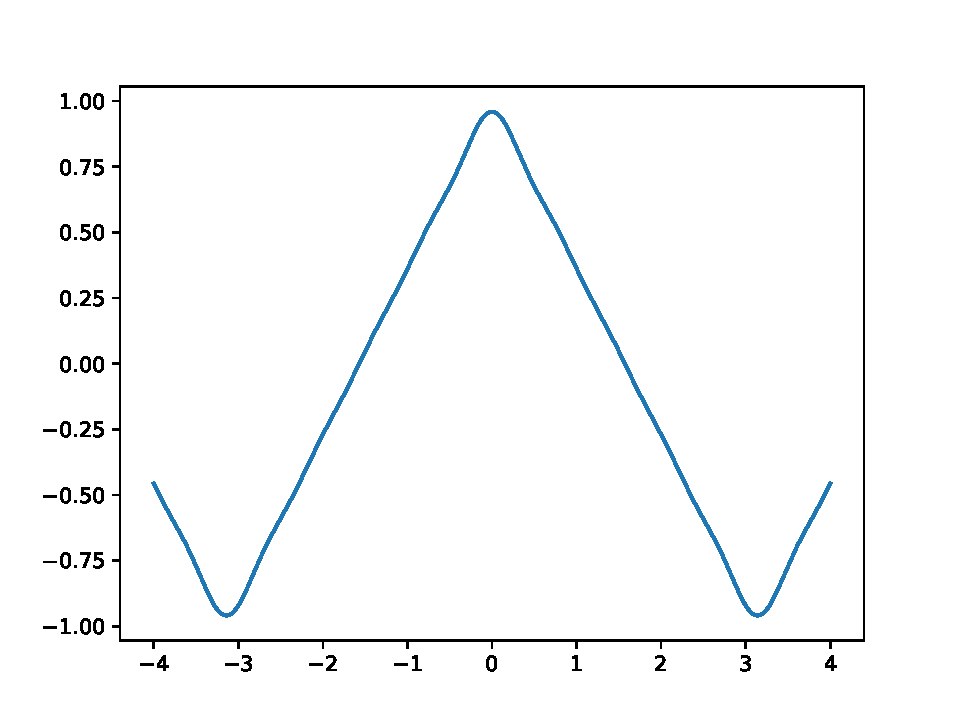
\includegraphics[]{plot/triangle}
	\caption{Сигнал <<треугольник>> по 100 первым гармоникам}
	\label{fig:figure1}
\end{figure}

%%%%%%%%%%%%%%%%%%%%%%%%%%%%%%%%%%%%%%%%%%%%%%%%%%%%%%%%%%%%%%%%%%%%%%%%%%%%%%%
\subsubsection{Пила}
\begin{equation}
	U(t)=\left\{
	\begin{aligned}
		0, \quad &t\in [-\frac{T}{2},0]\\
		\frac{2U_0}{T}t, \quad &t\in[0, \frac{T}{2}]
	\end{aligned}
	\right.
\end{equation}
\begin{equation}
	a_n=\frac{2}{T}\left[\int\limits_{\frac{T}{2}}^0 0\cdot\cos{(n\Omega t)} dt+\frac{2U_0}{T}\int\limits_0^{\frac{T}{2}}t\cdot\cos(n\Omega t)dt \right]=...=\frac{U_0}{n^2\pi^2}\cdot(\cos(\pi n)-1)
\end{equation}
\begin{equation}
	b_n=\frac{2}{T}\left[\int\limits_{-\frac{T}{2}}^00\cdot\sin(n\Omega t)dt + \frac{2U_0}{T}\int\limits_0^{\frac{T}{2}}t\cdot\sin(n\Omega t)dt\right]=...=\frac{U_0}{n\pi}\cdot(-1)^{n+1}
\end{equation}
\begin{equation}
	a_0=\frac{2}{T}\left[\int\limits_{\frac{T}{2}}^0 0\cdot dt+\frac{2U_0}{T}\int\limits_0^{\frac{T}{2}}t \,dt \right]=...=\frac{U_0}{2}
\end{equation}
% Даня $a_0$ не посчитал, ну и пёс с ним. Зато посчитал Федя. Напишу сразу разложение
\begin{equation}
	U(t)=\frac{U_0}{4}+\sum_{n=1}^{\infty}\left[\frac{U_0}{\pi^2n^2}\left((-1)^n-1\right)\cdot\cos(n\Omega t)+ (-1)^{n+1}\frac{U_0}{\pi n}\cdot\sin(n\Omega t)\right]
\end{equation}
\begin{figure}[tb]
	\centering
	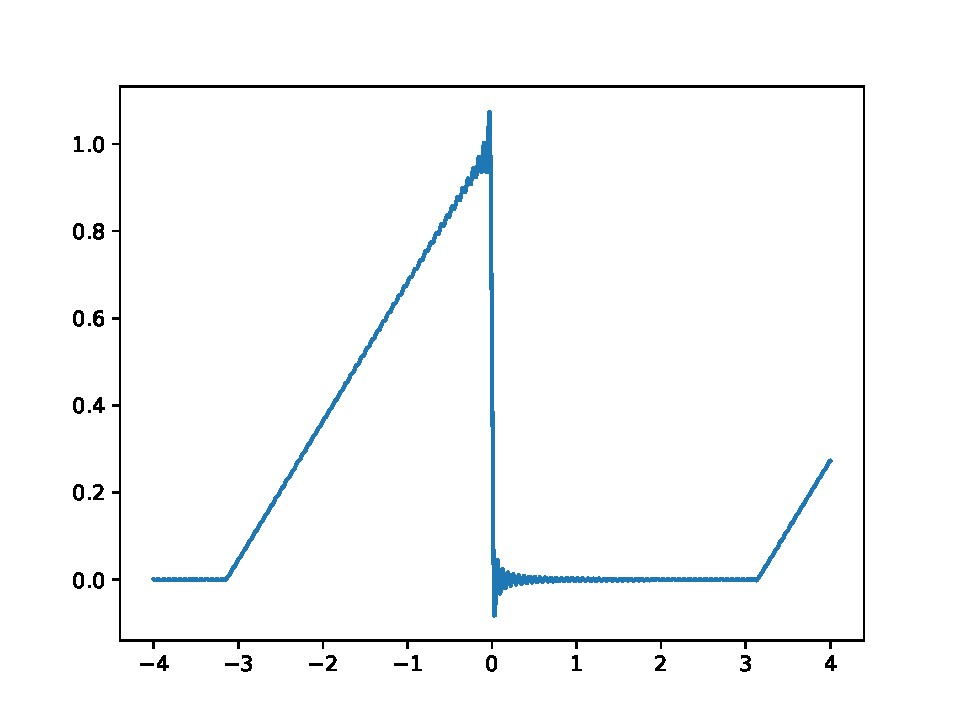
\includegraphics[]{plot/pila}
	\caption{Сигнал <<пила>> по 100 первым гармоникам}
	\label{fig:figure1}
\end{figure}

%%%%%%%%%%%%%%%%%%%%%%%%%%%%%%%%%%%%%%%%%%%%%%%%%%%%%%%%%%%%%%%%%%%%%%%%%%%%%%%
\subsubsection{Меандр}
\begin{equation}
	U(t)=\left\{
	\begin{aligned}
		-U_0,\quad &t\in [-\frac{T}{2},0]\\
		U_0,\quad &t\in[0, \frac{T}{2}]
	\end{aligned}
	\right.
\end{equation}
В силу нечетности $a_n\equiv 0$.
\begin{equation}
	b_n=\frac{4U_0}{T}\int\limits_{0}^{T/2} \sin(n\Omega t)dt=\frac{2U_0}{\pi n}(1-\cos(\pi n))
\end{equation}
И тогда
\begin{equation}
	U(t)=\sum_{n=1}^{\infty}\frac{2U_0}{\pi n}(1-(-1)^n)\cdot\sin(n\Omega t)
\end{equation}
\begin{figure}[tb]
	\centering
	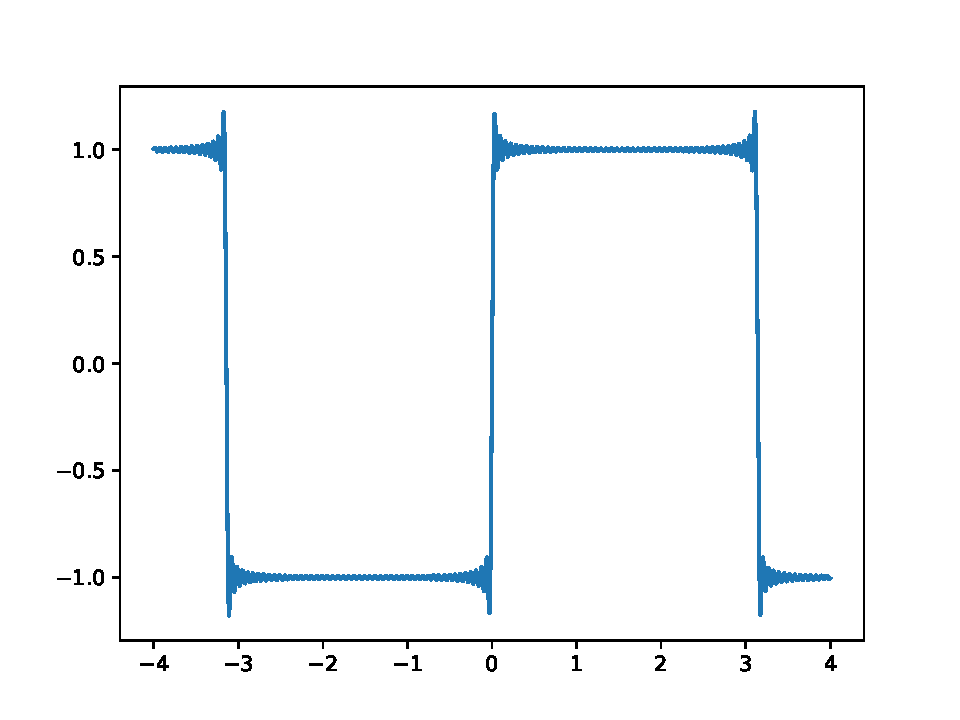
\includegraphics[]{plot/meandr}
	\caption{Сигнал <<меандр>> по 100 первым гармоникам}
	\label{fig:figure1}
\end{figure}

%%%%%%%%%%%%%%%%%%%%%%%%%%%%%%%%%%%%%%%%%%%%%%%%%%%%%%%%%%%%%%%%%%%%%%%%%%%%%%%
\newpage
\subsection{Спектры сигналов с установки}
\begin{figure}[H]
	\centering
	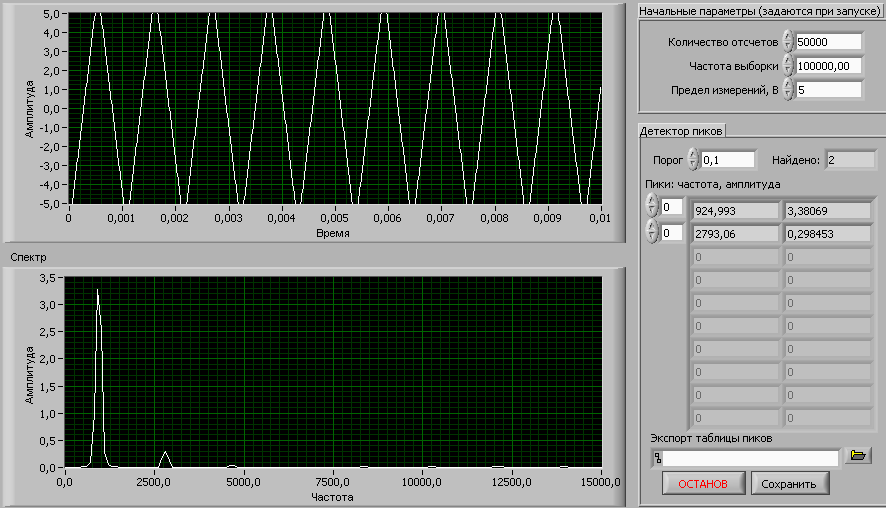
\includegraphics[width=0.85\textwidth]{pic/sig/triangle.png}
	\caption{Сигнал <<треугольник>>}
	
\end{figure}
\begin{figure}[H]
	\centering
	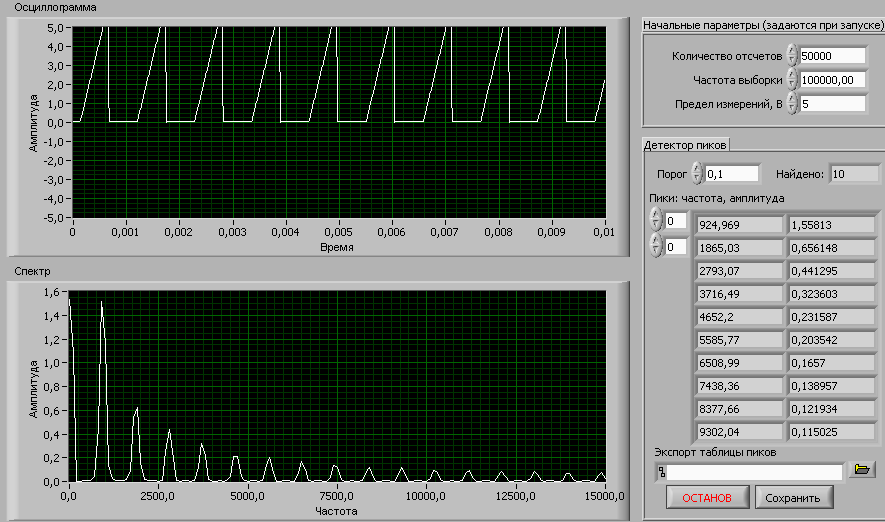
\includegraphics[width=0.85\textwidth]{pic/sig/pila.png}
	\caption{Сигнал <<пила>>}
	
\end{figure}
\begin{figure}[H]
	\centering
	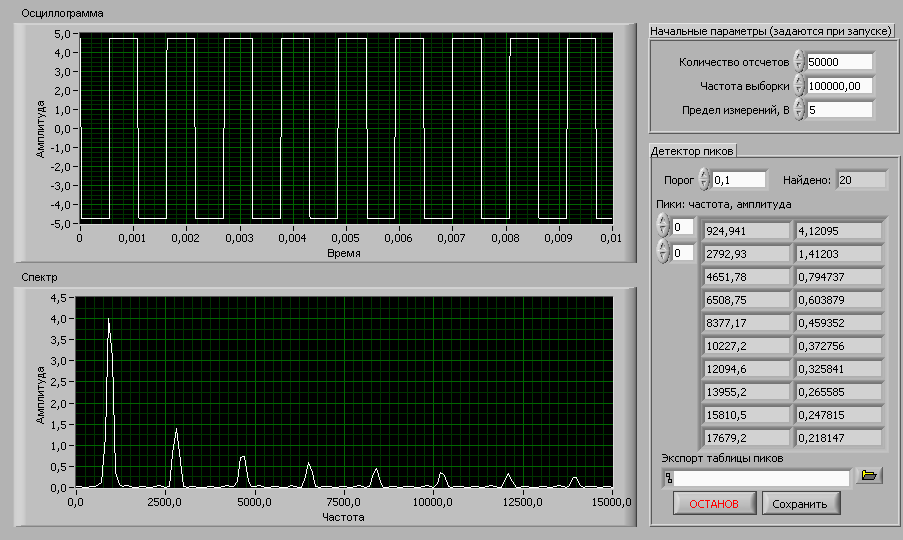
\includegraphics[width=0.85\textwidth]{pic/sig/meandr.png}
	\caption{Сигнал <<меандр>>}
\end{figure}

\subsection{Синтезированные сигналы}
\begin{figure}[H]
	\centering
	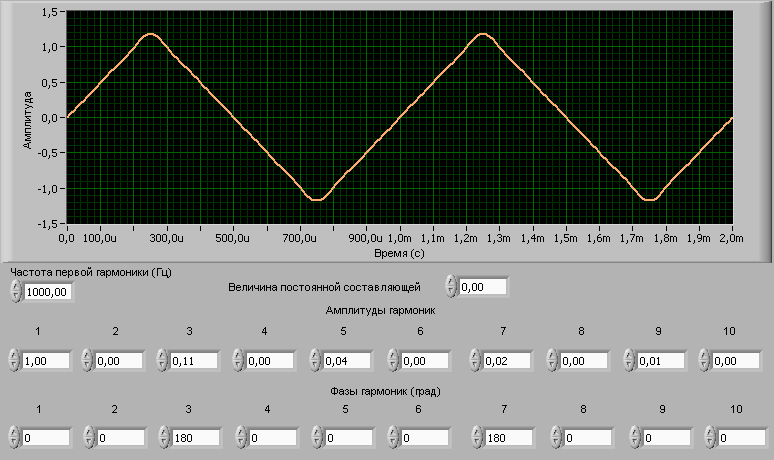
\includegraphics[width=0.85\textwidth]{pic/sint/triangle.png}
	\caption{Сигнал <<треугольник>>}
	
\end{figure}
\begin{figure}[H]
	\centering
	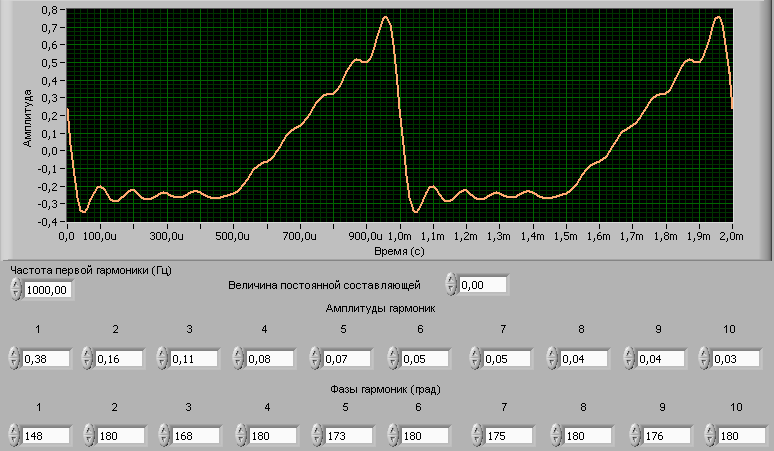
\includegraphics[width=0.85\textwidth]{pic/sint/pila.png}
	\caption{Сигнал <<пила>>}
	
\end{figure}
\begin{figure}[H]
	\centering
	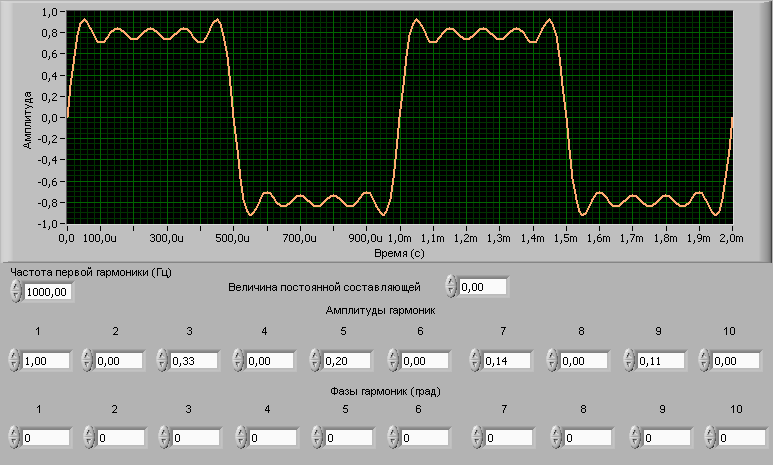
\includegraphics[width=0.85\textwidth]{pic/sint/meandr.png}
	\caption{Сигнал <<меандр>>}
	
\end{figure}

\subsection{Синтез амплитудно-- и частотно-- модулированных сигналов}
\begin{figure}[H]
	\centering
	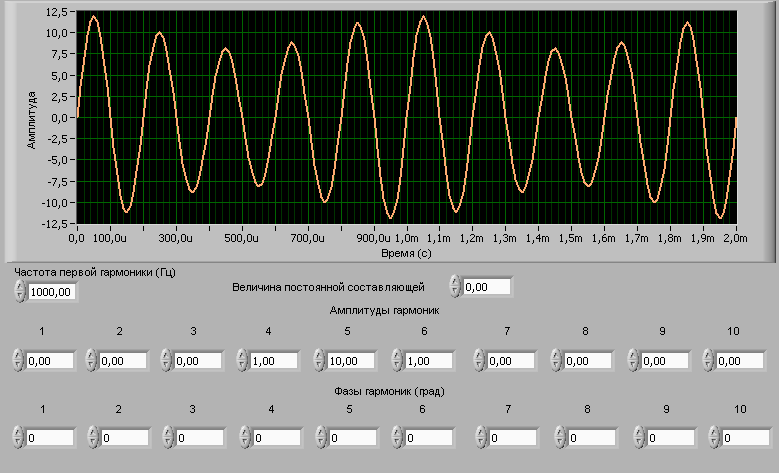
\includegraphics[width=0.85\textwidth]{pic/mod/mod2.png}
	\caption{Амплитудная модуляция с $m=0.20$}
\end{figure}
\begin{figure}[H]
	\centering
	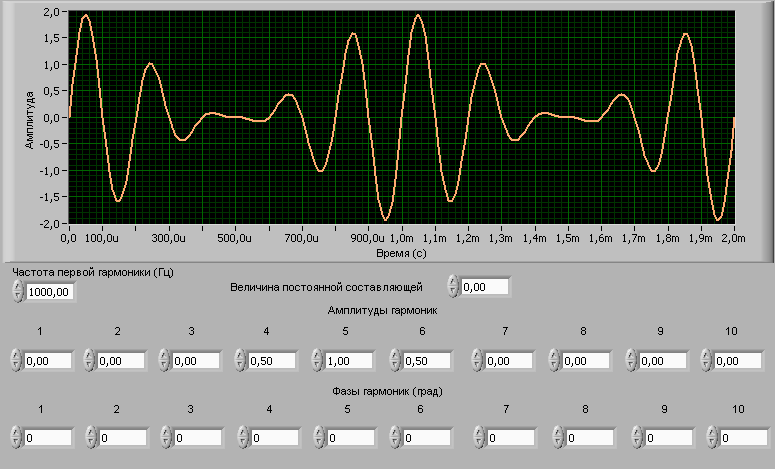
\includegraphics[width=0.85\textwidth]{pic/mod/mod1.png}
	\caption{Амплитудная модуляция с $m=1$}
\end{figure}
\begin{figure}[H]
	\centering
	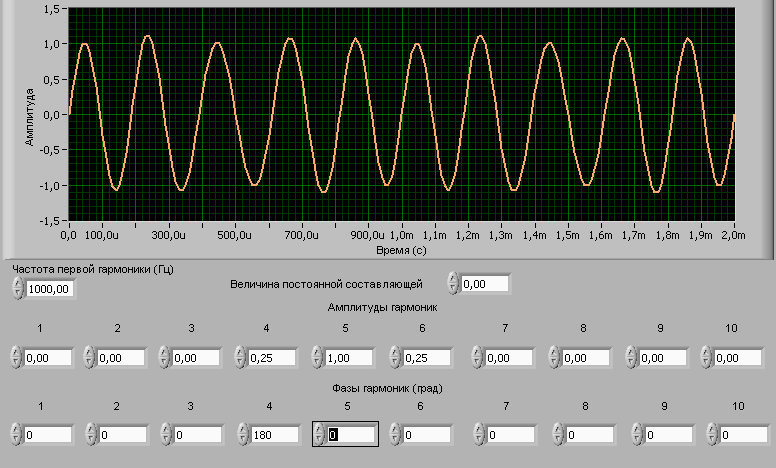
\includegraphics[width=0.85\textwidth]{pic/mod/mod3.png}
	\caption{Фазовая модуляция с  $m=0.25$}
\end{figure}
\begin{figure}[H]
	\centering
	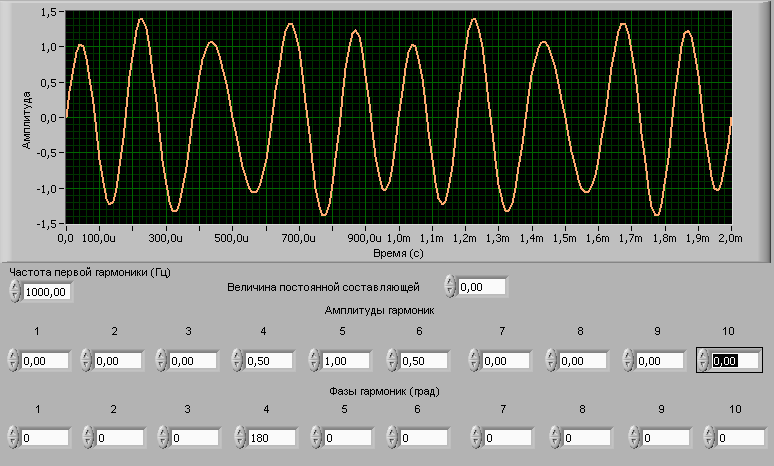
\includegraphics[width=0.85\textwidth]{pic/mod/mod4.png}
	\caption{Фазовая модуляция с  $m=1$}
\end{figure}
\subsection{Форма сигналов при дифферинцировании и интегрировании}
\subsubsection{Интегрированные сигналы}

\begin{figure}[H]
	\centering
	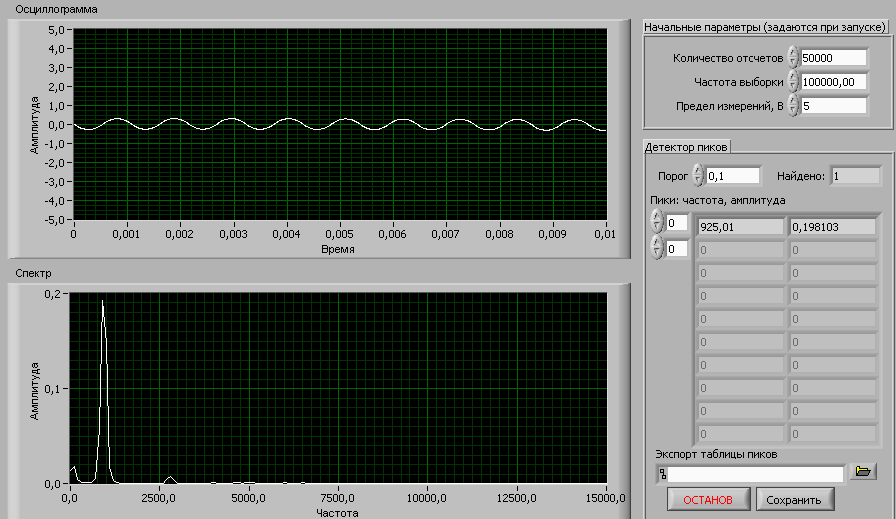
\includegraphics[width=0.85\textwidth]{pic/int/triangle.png}
	\caption{Сигнал <<треугольник>>}
	
\end{figure}
\begin{figure}[H]
	\centering
	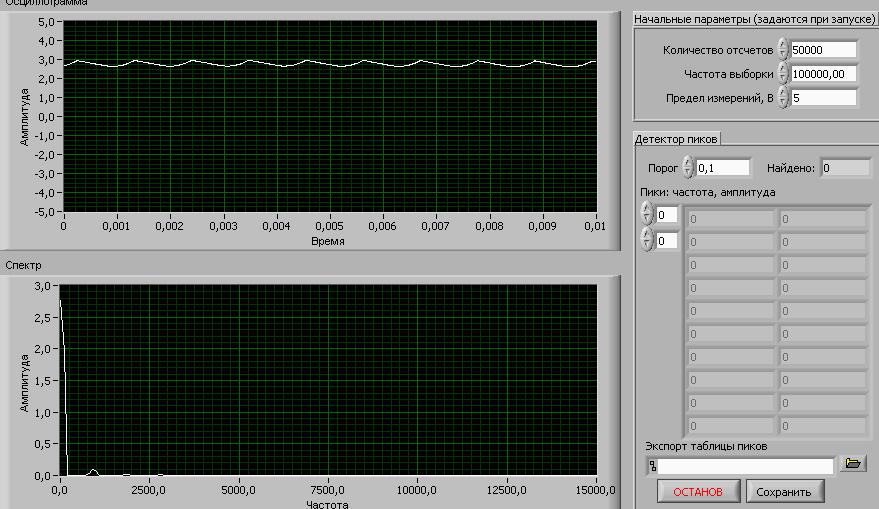
\includegraphics[width=0.85\textwidth]{pic/int/pila.png}
	\caption{Сигнал <<пила>>}
	
\end{figure}
\begin{figure}[H]
	\centering
	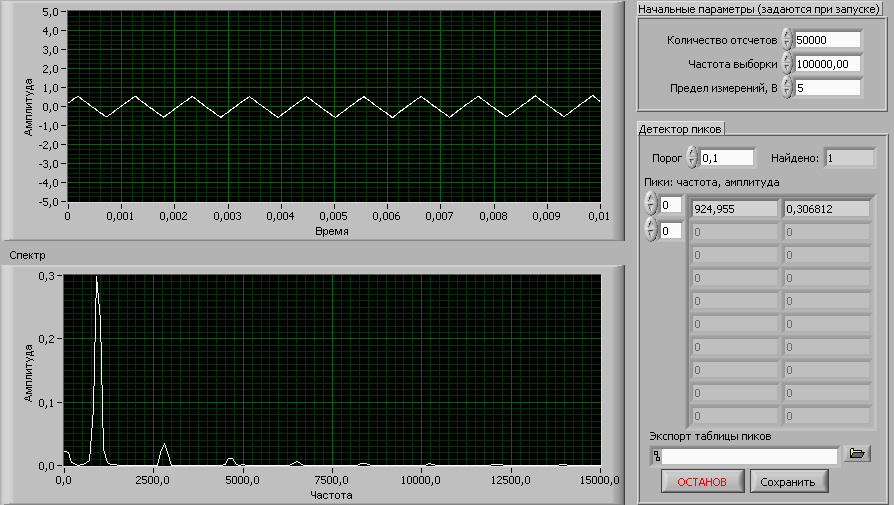
\includegraphics[width=0.85\textwidth]{pic/int/meandr.png}
	\caption{Сигнал <<меандр>>}
	
\end{figure}

% \paragraph{Некоторые значения $\tau=RC$}

\begin{figure}[H]
	\centering
	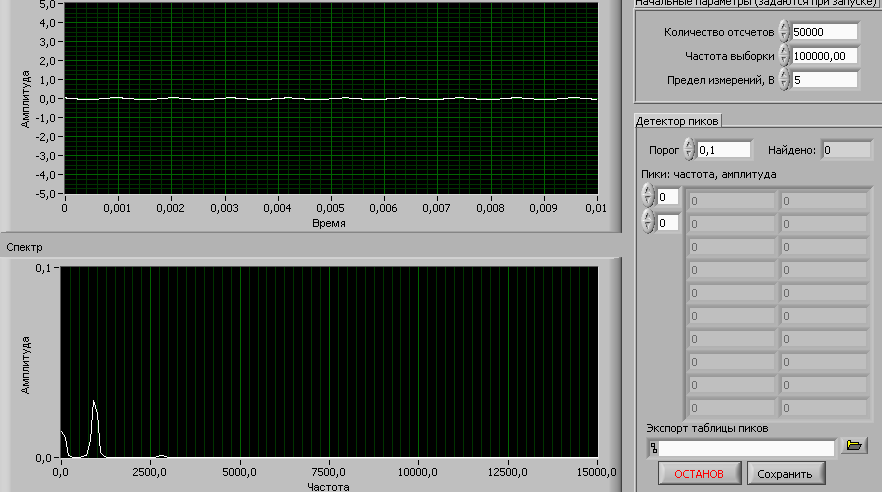
\includegraphics[width=0.85\textwidth]{pic/int/triangle_r_1000_c_50000.png}
	\caption{Сигнал <<треугольник>>, $R=1000$ Ом, $C=50000$ пкФ}
\end{figure}
\begin{figure}[H]
	\centering
	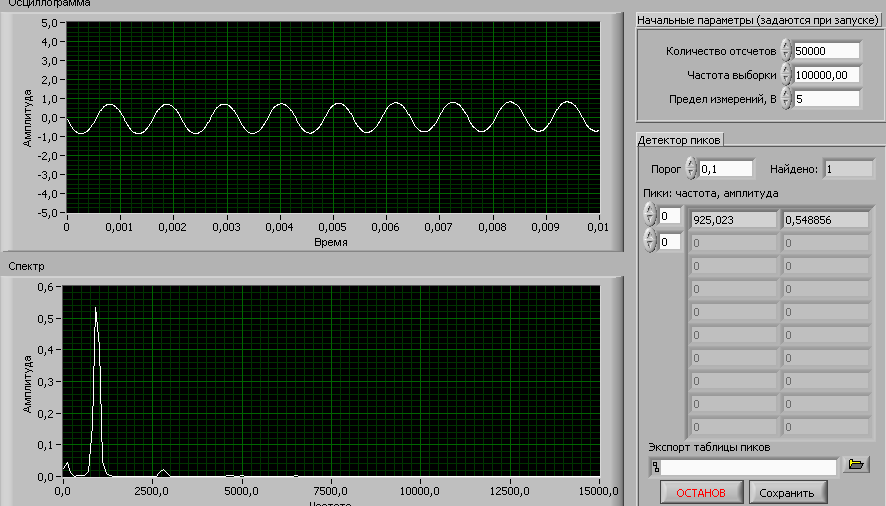
\includegraphics[width=0.85\textwidth]{pic/int/triangle_r_1000_c_5000.png}
	\caption{Сигнал <<треугольник>>, $R=1000$ Ом, $C=5000$ пкФ}
\end{figure}

\subsubsection{Дифференцированные сигналы}

\begin{figure}[H]
	\centering
	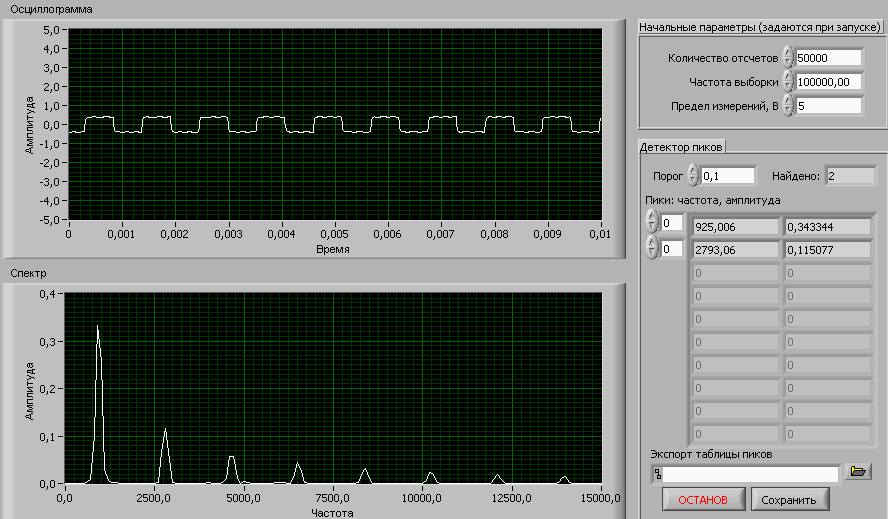
\includegraphics[width=0.85\textwidth]{pic/diff/triangle.png}
	\caption{Сигнал <<треугольник>>}
	
\end{figure}
\begin{figure}[H]
	\centering
	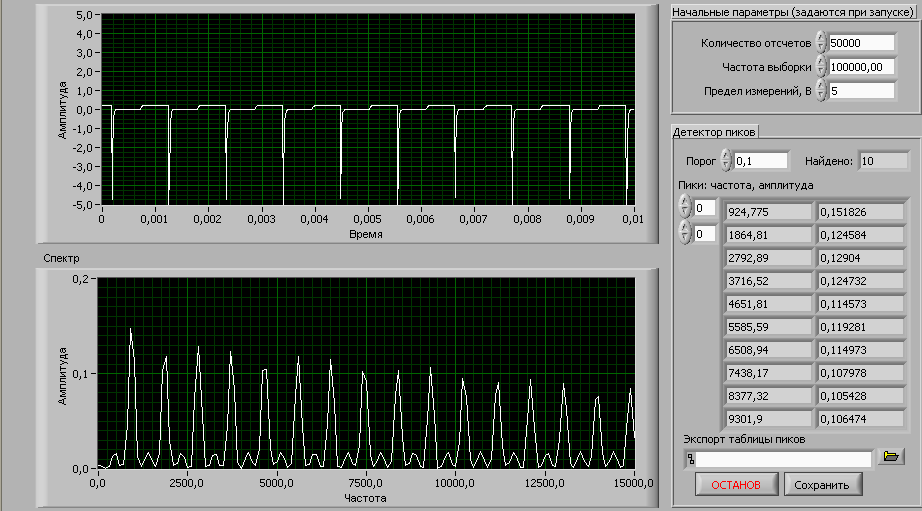
\includegraphics[width=0.85\textwidth]{pic/diff/pila.png}
	\caption{Сигнал <<пила>>}
	
\end{figure}
\begin{figure}[H]
	\centering
	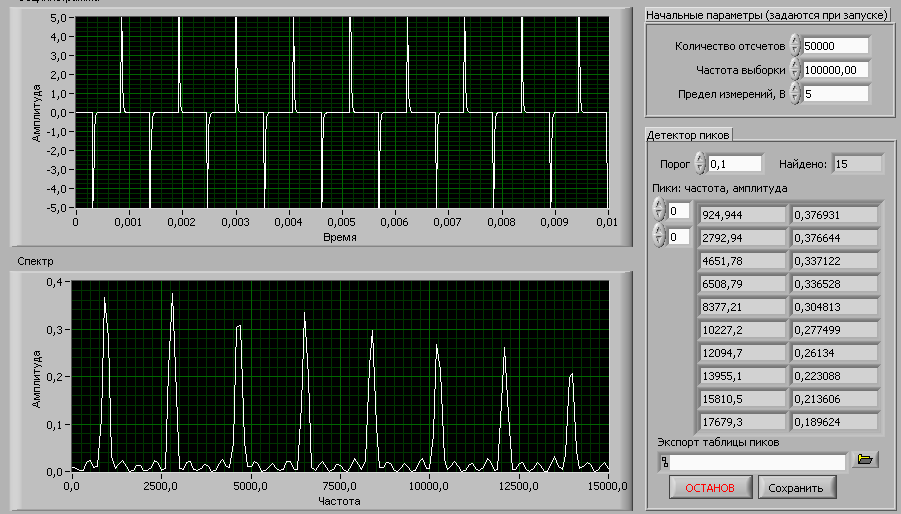
\includegraphics[width=0.85\textwidth]{pic/diff/meandr.png}
	\caption{Сигнал <<меандр>>}	
\end{figure}



% \section{Заключение}

\end{document}